
% this file is called up by thesis.tex
% content in this file will be fed into the main document
%----------------------- introduction file header -----------------------
%%%%%%%%%%%%%%%%%%%%%%%%%%%%%%%%%%%%%%%%%%%%%%%%%%%%%%%%%%%%%%%%%%%%%%%%%
%  Capítulo 1: Introducción- DEFINIR OBJETIVOS DE LA TESIS              %
%%%%%%%%%%%%%%%%%%%%%%%%%%%%%%%%%%%%%%%%%%%%%%%%%%%%%%%%%%%%%%%%%%%%%%%%%

\chapter{Introducción}

%: ----------------------- HELP: latex document organisation
% the commands below help you to subdivide and organise your thesis
%    \chapter{}       = level 1, top level
%    \section{}       = level 2
%    \subsection{}    = level 3
%    \subsubsection{} = level 4
%%%%%%%%%%%%%%%%%%%%%%%%%%%%%%%%%%%%%%%%%%%%%%%%%%%%%%%%%%%%%%%%%%%%%%%%%
%                           Presentación                                %
%%%%%%%%%%%%%%%%%%%%%%%%%%%%%%%%%%%%%%%%%%%%%%%%%%%%%%%%%%%%%%%%%%%%%%%%%
 % section headings are printed smaller than chapter names


\lettrine[lines=1]{L}as galaxias son sistemas complejos, de muchas componentes. Por lo general, una galaxia puede constar
de cientos de millones o miles de millones de estrellas, puede contener cantidades considerables de gas
y polvo interestelar, además puede estar sujeto a influencias ambientales a través de interacciones con otras galaxias
y con el gas inter-galáctico. La formación de estrellas tiene lugar en regiones densas de gas interestelar.
Para complicar más las cosas, la materia oscura está presente en las galaxias y en cúmulos de ellas, además de que
su masa es considerablemente mayor que la masa de la materia bariónica. En consecuencia, la dinámica de las galaxias
está dominada por esta componente oscura e invisible, cuya naturaleza hasta la fecha se desconoce.

\bigskip

\noindent Tradicionalmente, las galaxias se clasifican por estudios morfológicos. Estos esquemas de clasificación tienen que abarcar una
gran cantidad de detalles y esto se reflejó en los trabajos pioneros de Hubble \citep{hubble1936}.
La secuencia que Hubble introdujo, es básica en  astrofísica ya que una serie de propiedades físicas están correlacionadas con la morfología. Mientras que el estudio detallado de galaxias individuales era factible para estas cuestiones, un nuevo enfoque
tuvo que adoptarse para los \textsl{surveys} de galaxias, como por ejemplo, el \textsl{Sloan Digital Sky Survey} (SDSS) \citep{york2000},
que proporcionaron enormes bases de datos para estudiar una gran cantidad  de galaxias y así obtener sus propiedades estadísticas. Como resultado, los sistemas de clasificación se realizaron sobre la base de parámetros que pudieran derivarse del análisis de imágenes de galaxias y sus espectros existentes. En las secciones siguientes se dará un esquema  del conocimiento general que tenemos sobre estas y que nos ayudarán a entender el problema de UGC11680 como una galaxia espiral de color rojo.

\section{Clasificación de Hubble}

Las galaxias tienen una amplia variedad de diferentes morfologías. Edwin Hubble propuso cierto orden a esta diversidad en sus estudios
pioneros sobre las propiedades de estas como sistemas extra-galácticos \citep{hubble1936}. Ordenó a las galaxias en lo que
llegó a ser conocido como la secuencia de Hubble, distinguiendo las de apariencia elíptica, las galaxias elípticas o $E$, hasta las
espirales $S$, como se ilustra esquemáticamente en el diagrama de ``bifurcación'' en la Figura \ref{tuningfork}.

\begin{figure}
  \centering
    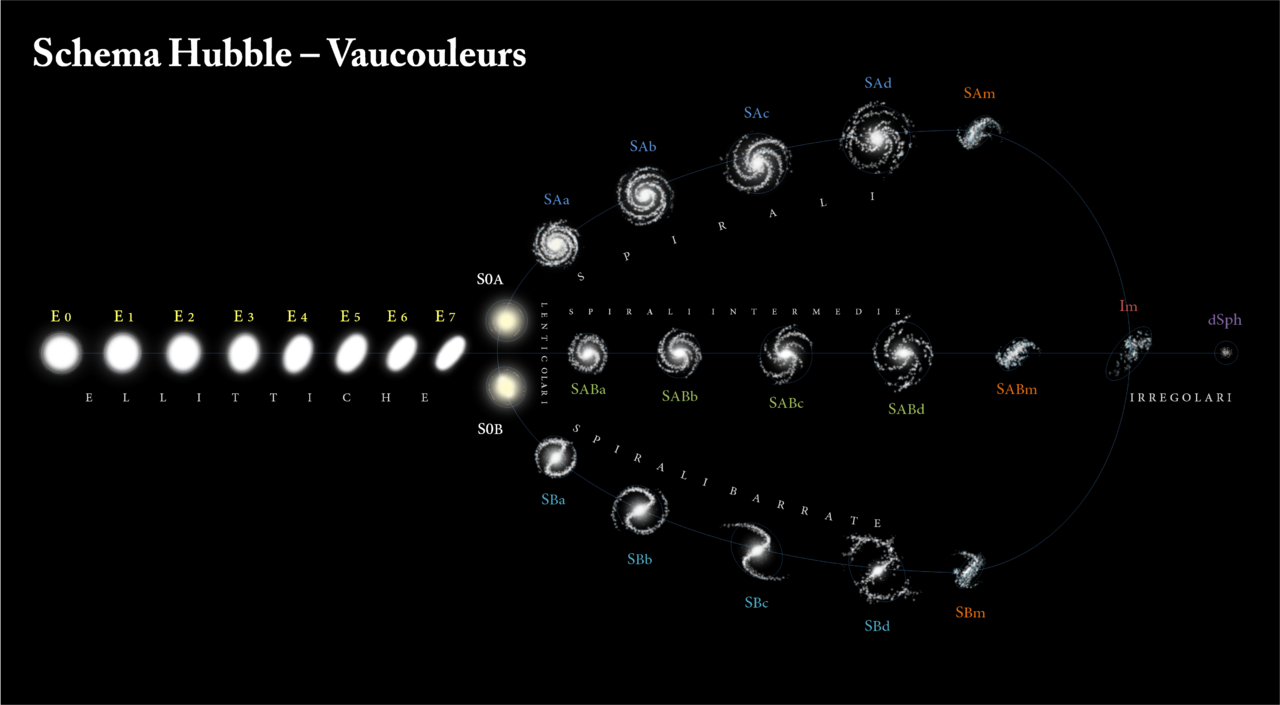
\includegraphics[scale=0.6]{hubble_mod.png}
  \caption[Diagrama de Hubble]{Diagrama de bifurcación mostrando la clasificación de Hubble con las modificaciones propuestas por De Vaucouleurs.}
  \label{tuningfork}
\end{figure}

\bigskip

\noindent Para las galaxias elípticas, el número $n$ después de la $E$ describe la elipticidad de la imagen, $n = 10 \times (a - b) / a$,
donde $a$ y $b$ son los ejes mayor y menor, respectivamente. De Vaucouleurs  propuso que las clases $Sd$ y $SBd$
deberían ser incluidas a la derecha de la secuencia y que las galaxias irregulares deben ser mostrada aun más a la derecha \citep{devaucouleurs1961}. Hubble creía que el diagrama de bifurcación era una secuencia evolutiva, por lo que para las elípticas, todavía se utiliza el término que propuso,``galaxias de tipo temprano'', mientras que para las espirales e irregulares les llamó consecuentemente, galaxias de tipo tardío. \footnote{ En este trabajo, se usará indistintamente estos términos por coherencia con la literatura, sin embargo, se debe recordar que solo son nombres históricos sin ninguna relación evolutiva.}


\bigskip

\noindent Las galaxias espirales están representadas en la ramas del diagrama bifurcación y se señalan con la letra $S$; las de la rama inferior son las  galaxias llamadas  espirales barradas, denotadas con el sigla $SB$. La letra minúscula después de la $S$ se basa en la apariencia de la estructura en espiral. $Sa$ y $SBa$ representa galaxias con brazos reforzados muy difusos y sus núcleos son grandes y luminosos. $Sb$ y $SBb$ caracterizan a las galaxias con brazos expandidos y pocos densos, con un pequeño bulbo. $Sc$ y $SBc$ son galaxias que tienen los brazos extendidos y pocos densos, con un bulbo aún menos brillante. Por último, las galaxias que marcan el punto de inflexión en el diagrama de bifurcación son las lenticulares y se denotan como $S0$. Estas galaxias se componen de un bulbo central y una estructura extendida en forma de disco que rodea a este bulbo. Las galaxias irregulares no tienen una estructura particular, se denotan con la sigla $Irr$ y la característica principal es que estas son asimétricas, sin bulbo central o sin espiral. En la clasificación ampliada, se colocan al final de la rama de las galaxias espirales.



\section{AGNs}

Dentro de ambos tipos (espirales ó elípticas) existen algunas que muestran un centro muy luminoso, del orden de $L \sim 10^{10} L_{\odot}$. A estas galaxias se les denominó como ``galaxias activas'' o actualmente como ``Núcleos Activos Galácticos'' (AGNs).
La característica principal que distingue a estos objetos de las galaxias inactivas (normales o regulares) es
la presencia de agujeros negros super-masivos que acretan materia en sus centros. Hasta la fecha, hay aproximadamente un millón de fuentes
conocidas de este tipo, seleccionado por su color y varios cientos de miles por espectroscopía \citep{santini2012}.

\bigskip

\noindent Se estima que en el Universo Local, a un \textsl{redshift} de $z \sim 0.1$, aproximadamente 1 de cada 50
galaxias contiene una hoyo negro super-masivo con rápida acreción, y aproximadamente 1 de cada 3
contiene uno de lenta acreción (\cite{richards2006}; \cite{rosario2012}). Los estudios detallados de grandes muestras de AGNs, la comprensión de su relación con las galaxias inactivas y su evolución con respecto al \textsl{redshift} comenzó a finales
1970, mucho después del descubrimiento de los primeros objetos cuasi-estelares (en lo sucesivo, cuásares) a principios de 1960.

\bigskip

\noindent  Debido a su importancia histórica, los primeros nombres que se les dieron a estos objetos, recuerdos de los años 60's y 70's, (e incluso más tarde) todavía se utilizan. Algunos de los nombres que aparecen ocasionalmente en la literatura, tales como ``Seyfert 1'' y ``Seyfert 2'', (en honor de Carl Seyfert, quien observó las primeras galaxias de este tipo
a finales de 1940), son el resultado de una de las primeras confusiones entre diferentes fuentes que ahora se sabe tienen propiedades similares. La principal diferencia observacional entre las \textsl{Seyfert} 1 y \textsl{Seyfert} 2 es su espectro  en el óptico-ultravioleta (UV).
Las \textsl{Seyfert} 1  muestran líneas permitidas muy fuertes y anchas ($\sigma$ $\sim$ 2000-10,000 km/s si se interpreta como ensanchamiento Doppler), mientras que las líneas en las \textsl{Seyfert} 2  tienen anchos que no exceden  $\sim$ 1200 km/s.

\bigskip

\noindent Tales diferencias ahora se entienden como el resultado de diferentes ángulos de visión a los centros de dichas fuentes y
también en parte, debido a una gran cantidad de oscurecimiento a lo largo de este. La nomenclatura común que se utilizará a lo largo de esta tesis es de AGN tipo I  para las fuentes que presenten una linea de visión despejada de sus centros y AGN tipo II para objetos afectados con oscurecimiento a lo largo la línea de visión que  extingue toda la radiación óptica-UV del interior. Las observaciones de los núcleos galácticos activos, (y otro ejemplo de clasificación) era la tendencia por separar el AGN según su luminosidad \citep{urry1995}. El nombre de ``galaxias Seyfert'' fue reservado para objetos de baja luminosidad, en su mayoría AGNs con bajo \textsl{redshift}, mientras que se llamó \textsl{QSO} a los miembros más luminosos de la familia. De hecho, la línea divisoria  entre galaxias \textsl{Seyfert} y cuásares no es muy precisa; algunos investigadores sugieren que la línea debe establecerse en alrededor de
$L_{bol}=10^{45}$ erg/s, donde $L_{bol}$ es la luminosidad  bolométrica de la fuente central \citep{antonucci1993}.

\bigskip

\noindent Otros prefieren una división basada en \textsl{redshift}, por ejemplo, en algunos trabajos todos los AGN con
$z \sim 0.2$ se consideran  cuasáres \citep{vanden2001}. Para añadir mas complejidad (o confusión), varios nombres se han propuesto en los últimos años para los AGNs con diferencias observacionales y propiedades físicas que  los originan: ``N-galaxias'', radio-galaxias de líneas anchas ``(BLRGs)'', radio-galaxias de línea angosta ``(NLRGs)'', galaxias en rayos
X con línea de emisión angosta``(NLXGs)'', objetos BL-Lac, QSO variable ópticamente violento ``(OVVs)'',
y  regiones de líneas de emisión de baja ionización nuclear  ``(LINERs)'' entre otros.
Para no entrar en confusiones, en este trabajo optaremos por utilizar el nombre genérico ``AGN''.

\bigskip

\noindent De este modo, podemos basar nuestra  definición de  actividad nuclear en galaxias
dada  por la huella observacional de esta actividad. Entonces, la definición
que usaremos es simple: un objeto extra-galáctico se considera que es un AGN sí
contiene una hoyo negro con acreción en su centro y sí se cumple al menos una de las siguientes características:

\begin{itemize}

\item Contiene una región nuclear compacta con emisión significativa, más allá de lo
se espera de los procesos estelares típicos de este tipo de Galaxias.

\item Se muestra la huella clara de un proceso continuo no estelar en emisión en
su centro.

\item Su espectro contiene fuertes líneas de emisión con relaciones de líneas que son típicos de
excitación por radiación no estelar.

\item Variaciones de líneas de emisión y/o del continuo.
\end{itemize}




\section{Bimodalidad}

Una vez establecida la existencia de los AGNs y su relación con el núcleo activo en cualquier tipo morfológico de galaxia,
 ya sea espiral o elíptica, regresamos  al tema de la morfología, la diferencia más notable en galaxias,visualmente hablando.
Las galaxias de diferente morfología presentan propiedades claramente diferenciadas, como en color (azul vs. rojo), en cinemática (soportado por presión o rotación), en luminosidad típica (menores vs. superiores),
en la agrupación con otras galaxias (menores vs. mayores entornos de densidad), etc. Muchas de estas diferencias son el resultado ó
se cree están relacionadas con las variaciones en el contenido de gas frío, que a su vez conducen a niveles diferentes de formación estelar. Las galaxias de tipo temprano, que incluyen elípticas y lenticulares ($S0$), fueron consideradas tradicionalmente como representantes de una población inactiva y son llamadas algunas veces como ``galaxias pasivas'' \footnote{También Conocidas equivalentemente en la literatura como \textsl{Quiescentes}}. La historia de formación de estas galaxias y otras de diferentes morfología, sigue siendo una de las cuestiones centrales en la investigación actual  \citep{perez2013} ;({\color{red} Ibarra-Medel, et.al. Submitted }).

\bigskip

\noindent Un salto importante para entender las diferencias en las propiedades de las galaxias debido a su morfología, se produjo con la llegada  del llamado  \textsl{Sloan Digital Sky Survey} (SDSS), \citep{york2000}. Con su gran muestreo espectroscópico de galaxias en el Universo Local, ($z \sim 0.1$, \cite{strauss2002}) además de su fotometría óptica en cinco bandas; el SDSS permitió el análisis estadístico de estas poblaciones. De esta forma se logró clasificar a una gran cantidad de galaxias en un diagrama que llamamos de color-magnitud (CMD) y este corroboró que las galaxias de campo forman dos ``picos'' en la distribución de color en el óptico \cite{strateva2001}; \cite{baldry2004}. El pico estrecho rojo ya había sido estudiada previamente en cúmulos de galaxias y era conocido como la \textsl{secuencia roja} \citep{devaucouleurs1961}.

\bigskip

\noindent El SDSS confirmó además que la secuencia roja, y en consecuencia las tempranas que se encuentran en ella, son abundantes en
ambientes aislados \citep{butcher1984}. El pico más amplio en la banda azul del óptico
se nombró como la nube azul. Las diferencias físicas entre las dos poblaciones
se exploraron a fondo y se cuantificaron por \cite{kauffmann2003}, quien encontró que las
galaxias en la secuencia roja tienen, en promedio, las poblaciones estelares de mayor edad,
mayor densidad de masa estelar superficial, y dominan a masas estelares mayores a $ \sim 10^{10.5} M_{\odot}$.


\bigskip

\noindent Esta bimodalidad de las distribuciones de color se convirtió no solo en un punto central en los estudios de galaxias locales, sino también con \textsl{redshifts}  mayores. \cite{bell2004} y \cite{faber2007} reportaron que la función de luminosidad de las galaxias de la secuencia roja se ha incrementado en un factor de dos o más desde $z \sim 1$. Este resultado sugiere que la acumulación de masa de las galaxias en la secuencia roja (y así posiblemente de galaxias tempranas) es un proceso que está en curso ($\sim$ 8 Gyrs). Este escenario estaría en desacuerdo con la imagen tradicional en el que las tempranas (especialmente elípticas) se formaron
en épocas muy tempranas en la historia del universo (es decir, deteniendo su formación estelar y convirtiéndose en galaxias de color rojo).

\bigskip


\noindent Esta imagen tradicional, tiene sus raíces en el escenario de colapso monolítico propuesto por \cite{eggen1962}, que posteriormente fue sustituido por el escenario jerárquico (por ejemplo \cite{kaufmann2006}) en el que las fusiones de las galaxias de disco proporcionan un mecanismo natural de formación de las galaxias elípticas \citep{barnes1996}. Si las fusiones siguen siendo importantes en las últimas épocas del universo, como algunas simulaciones numéricas sugieren, entonces se abriría la puerta para la formación tardía de galaxias elípticas y explicaría el crecimiento reportado de la secuencia roja.

\bigskip

\noindent Además, si las galaxias tempranas se continúan formando hasta épocas cosmológicas recientes, entonces  deberían existir galaxias que se encuentren actualmente en un proceso de transformación. Este tipo de galaxias tienen (o deberían tener) propiedades que estén entre las galaxias tardías y las galaxias de tipo temprano. Por ejemplo, deben tener algo de formación estelar, pero la mayor parte de la actividad debería haber cesado, es decir, la tasa de formación estelar ($SFR$), debería sería menor que el de las galaxias de tipo tardío de la misma masa. Por lo tanto, ¿cómo  puede identificarse tal población transitoria a gran escala?

\subsection{El Valle Verde}

Podemos definir al Valle verde como una región amplia y relativamente plana
(por lo tanto, `` valle") en el diagrama color-magnitud de galaxias,
que se encuentra entre los picos formados por  galaxias con formación estelar (nube azul)
 y las galaxias pasivas (secuencia roja). Además el valle verde
se ha propuesto  como el cruce en la evolución de las galaxias. Los
objetos en el valle verde se cree que representan la transición entre la nube azul de las galaxias de formación estelar y la
secuencia roja. ( \cite{kauffmann2003};\cite{wyder2007} ;\cite{schiminovich2007}; \cite{martin2007}; \cite{faber2007}; \cite{mendez2011}; \cite{goncalves2012}). En términos generales, se cree que todas las galaxias  siguen
trayectorias evolutivas similares en todo el valle verde, con una
rápida transición que explica la escasez relativa de las galaxias en el
valle verde en comparación con la nube azul o la secuencia roja \citep{haines2015}.

\bigskip

\noindent Los colores intermedios en el valle verde se
han interpretado como evidencia del apagado reciente de la formación de estrellas
\citep{salim2007}. La agrupación de
AGNs y sus galaxias huésped en el valle verde sugieren un papel más
para la retroalimentación del AGN en particular (por ejemplo,\cite{nandra2007}; \cite{hasinger2007}; \cite{silverman2008}; \cite{sanchez2004} ). Además, las galaxias en el valle verde tienen tasas de formación estelar (SFR) más bajas que la ``secuencia principal''
de formación de estrellas \citep{cano2016}, que es una correlación estrecha entre
la masa estelar y la tasa de formación de estrellas, posiblemente como resultado
de un apagado en la formación estelar  rápido (por ejemplo \cite{brinchmann2004}; \cite{elbaz2007};
\cite{salim2007}; \cite{noeske2007}; \cite{peng2010}).La mayoría de las galaxias de formación estelar
viven en la secuencia principal, por lo que el seguimiento de las poblaciones que salen de la
secuencia principal  (aquellos con bajos SFRs) se pueden utilizar para buscar el mecanismo de apagado en las mismas.

\section{Bimodalidad y Apagado en la Formación Estelar}

Hasta antes de la llegada de catálogos de galaxias espacialmente resueltas, la relación entre los mecanismos para la formación estelar y su apagado en galaxias se comprendía menos que hasta la fecha. Desde la perspectiva teórica, varios mecanismos de apagado en la formación estelar se propusieron, incluyendo por ejemplo:  el núcleo activo (AGN) y su retroalimentación (\cite{croton2006}; \cite{Hopkins2006}), \textsl{Shock Heating} en el halo (\cite{dekel2006}; \cite{cattaneo2006}), apagado  morfológico (\cite{martig2009}) y efectos de medio ambiente (\cite{gunn1972}; \cite{toomre1972}; \cite{moore1996}; \cite{bosselli2006}; \cite{weinmann2009}). Sin embargo, observacionalmente era extremadamente difícil identificar el mecanismo dominante. Por ejemplo, las galaxias masivas ($\sim$ $10^{11} M_{\odot}$ ) están preferentemente en regiones densas, es decir, efectos ambientales y por consiguiente el enfriamiento del halo podrían tener relación con estos procesos.

\bigskip


\noindent Para el caso de procesos internos, \citep{bluck2014} encuentran que el color (U-B) de una galaxia esta fuertemente ligada a una densa estructura interna y muestran además que la fracción inactiva está más estrechamente vinculada al bulbo. Dado la estrecha correlación entre la masa del bulbo y la masa del agujero negro, los autores sugirieron que la retroalimentación por AGN está más favorecida. Además, se sabe que muchas galaxias tienen una alta probabilidad de tener al mismo tiempo un bulbo con  AGN (\cite{kaufmann2006}; \cite{heckman2004}; \cite{schawinski2014}), lo que hace difícil aislar el efecto de una retroalimentación del AGN del bulbo central. Estas complejidades han obstaculizado en gran medida nuestro conocimiento del origen del apagado interno en formación estelar.

\section{El AGN como regulador de la formación estelar}

\noindent Una forma útil para seguir la evolución de galaxias observacionalmente es construir una función de luminosidad de todas las galaxias en un determinado \textsl{redshift}. La función de luminosidad $\Phi(L, z)$, se define de tal manera que $dN=\Phi(L, z) dVdL$ es el número de  galaxias por unidad de volumen co-movil, $dV$ a redshift $z$ en el intervalo de luminosidad
$L$, $L + dL$. El uso del volumen co-móvil, que se obtiene de la integración
del volumen entre $r(z)$ y $r(z + \Delta z)$ utilizando la cosmología supuesta, permite
una comparación directa de la misma población  en todos los \textsl{redshifts}.
Por lo tanto, $\Phi(L, z)$ proporciona una forma concisa para describir la evolución de galaxias en diferentes
tiempos cosmológicos \citep{kennicutt1998}.

\bigskip

\noindent Las luminosidades dependientes del \textsl{redshift} pueden ser comparadas con las predicciones teóricas que incluyen
solo enfriamiento bariónico simple. Dicha comparación muestra un ajuste entre el modelo y las observaciones para una amplia
gama de luminosidades alrededor de la $L_{*}$ . Sin embargo, el número calculado de galaxias más masivas ($\sim$ $10^{11}$ $M_{\odot}$) y las galaxias menos masivas ($\sim$ $10^{8}$ $M_{\odot}$) se desvían de las observaciones.
Por otra parte, hay una discrepancia significativa entre la predicción del enfriamiento atómico ya que debe llevar a la condensación
de alrededor del 80 por ciento de todos los
bariones \footnote{De vez en cuando usaremos la frase masa bariónica para referirnos a las simulaciones,
mientras que masa estelar define a las observaciones}
disponibles en gas y las estrellas en las galaxias. Sin embargo,las observaciones muestran que
esta fracción es inferior a 10 por ciento en $z = 0$.

\bigskip

\noindent Una posible solución es invocar un proceso de retroalimentación, es decir, un mecanismo que
inhiba el enfriamiento de gas y formación de estrellas en fases avanzadas de la formación de galaxias. Esto puede ser debido
a las estrellas ("retroalimentación estelar") o al AGN. Por
ejemplo, se piensa que en retroalimentación estelar la foto-ionización de
el gas bariónico en el halo puede retrasar la formación de galaxias pequeñas
en halos de materia oscura, lo que explica la falta de objetos en el extremo más bajo en la función de luminosidad.
Esto sin embargo, no puede explicar la falta de galaxias masivas $\sim 10^{11} M_{\odot}$ predichas por los modelos y otros procesos
de retroalimentación deben ser incluidos.


\bigskip

\noindent Como se mencionó, la correlación significativa entre la masa estelar (bulbo) y la masa del hoyo negro
en galaxias cercanas sugiere que la evolución del hoyo negro y la evolución de las galaxias van de la mano.
Esto plantea preguntas acerca la naturaleza de los procesos físicos que los enlazan, en particular, lo relacionado a que proceso
puede activar el hoyo negro central super-masivo  y apagar la formación estelar  en la galaxia huésped. Tal
proceso, si es lo suficientemente eficiente, pueden explicar la discrepancia entre las observaciones
con los cálculos de la función de luminosidad (en particular, la falta de grandes galaxias elípticas)
en comparación con las predicciones teóricas.

\bigskip

\noindent Esta retroalimentación se supone que puede venir en dos modos diferentes en épocas diferentes
durante el tiempo cósmico. En una fase temprana (a alto \textsl{redshift}) el
AGN puede apagar la formación de estrellas en las galaxias masivas. Es llamado el ``modo cuásar''
(\citet{croton2006}) y es más probable que venga acompañada de  un vigoroso
crecimiento lo que lleva a una fuerte retroalimentación cinética del agujero negro.
La otra forma de retroalimentación puede ser el AGN en ``modo regulador''. Este modo apaga la formación estelar en  épocas cosmológicas  recientes de tal manera que impide episodios significantes  de formación de estrellas \citep{fabian2006}. El acoplamiento entre la
acreción del agujero negro y el calentamiento  del gas esta limitados por lo dictado por las
observaciones .Sin Embargo, Si bien este tipo de hipótesis tienen éxito para subsanar algunas cuestiones clave, su principal problema es que la física de este proceso aún es poco conocido.

\section{Espirales Rojas: La Excepción a la Regla}

Como sucede en muchas ocasiones, existen excepciones a la regla y que nos obligan a cambiar el paradigma,
ya que se encontraron galaxias tardías o espirales con colores predominantemente rojos hace ya algún tiempo
(Por Ejemplo, \cite{bergh1976} sobre galaxias anémicas). El tamaño de su muestra era pequeño, sin embargo, quedo claro
que esos sistemas eran raros en el Universo Local. Esto implicaba que los procesos que llevaban a esos
objetos a ser rojos debían o ser raros, o producirlos solo por periodos cortos.
Cualquiera que fuera el motivo, estas espirales rojas eran  buenos laboratorios para estudiar
la evolución galáctica y comprender mejor como se ensamblaron las galaxias tempranas para formar la secuencia roja.

\bigskip

\noindent Otro de los proyectos interesantes que permitió una mejor comprensión de este grupo de galaxias es el famoso
\textbf{Galaxy Zoo}  (\cite{lintott2008})  que permitió distinguir una población significativa de espirales rojas (\cite{bamford2008}).
dentro de una selección de todas las galaxias espirales en general. Estos trabajos sugirieron que alrededor de 20 \% de esas galaxias se encuentran en la secuencia roja (y con una fracción creciente en regiones de densidad Media).
La fracción de espirales rojas parecía crecer con el medio ambiente, aún a masa estelar fija, implicando que algún proceso externo suprimía la formación de estrellas en las espirales rojas, mas allá de un simple cambio en la función de masa. (\cite{bamford2008})

\bigskip

\noindent Al mismo tiempo \citep{wolf2009} identificaron una muestra de espirales rojas y demostraron que estas tienen una tasa
de formación estelar (SFR) si bien baja, no era cero cuando se comparaba con las espirales azules.
Sin embargo, estos trabajos incluían espirales inclinadas. Esto como se sabe, puede hacer que galaxias azules se encuentren en la
secuencia roja debido a los efectos de enrojecimiento por polvo que depende de la inclinación (\citep{maller2009}, \citep{masters2010}).
También es bien sabido que las espirales con grandes bulbos pueden ser bastante rojas. Por ejemplo \citep{masters2010}
demostraron que esta tendencia en color debido al incremento en el bulbo es comparable en tamaño al enrojecimiento por inclinación.
Por esa razón \citep{masters2010} seleccionaron una nueva muestra de espirales de cara del \textsl{Galactic Zoo} con bulbos pequeños para
estudiar las propiedades  de espirales intrínsecamente rojas.
De esas espirales de cara, encontraron que alrededor del 6\% caen en la secuencia roja
(incrementando en 30\% cuando se incluían galaxias dominadas por bulbo). Además mostraron que sí bien tienen una tasa de formación estelar baja, no son objetos completamente pasivos (lo cual confirmó \cite{cortese2012}). La fracción de galaxias tardías en la secuencia roja se incrementaba sustancialmente con la masa estelar, pero a toda las masas estelares la población de espirales rojas parecían tener una población estelar más vieja y una menor formación estelar reciente que las espirales azules.

\bigskip

\noindent Mientras que las tardías rojas son relativamente raras en el Universo Local, estas podrían formar un camino importante para entender la evolución entre la nube azul y la secuencia roja. \citep{bundy2010} uso datos del COSMOS \textsl{survey} \citep{cosmos2007} para estudiar la secuencia roja de galaxias con morfología de disco a altos \textsl{redshifts} y concluyó que una cantidad significativa de galaxias con disco se traslada de la nube azul a la secuencia roja (60\%) pasando por una fase de espiral roja. \citep{robaina2012} comparó la población estelar de una muestra de galaxias con morfología espiral o elíptica y que fueron seleccionadas por su pasividad y su bajo enrojecimiento por polvo. Estas espirales rojas por definición, eran más pasivas que la muestra de \citep{masters2010} y además no hizo ninguna selección por el tamaño del bulbo. El trabajo de \citep{robaina2012} encontró que la población estelar en las dos muestras (en edad y metalicidad) eran estadísticamente indistinguibles.

 \section{UGC11680}

 La galaxia espiral UG11680 pertenece al tipo de galaxias tardías que se menciona en la sección anterior. Su color rojo podría ser
 indicador de que ha dejado de formar estrellas y aún conservar su morfología espiral, por lo que puede ser un laboratorio para analizar
 el proceso que llevo a ese color.

 \begin{figure}[!ht]
   \centering
   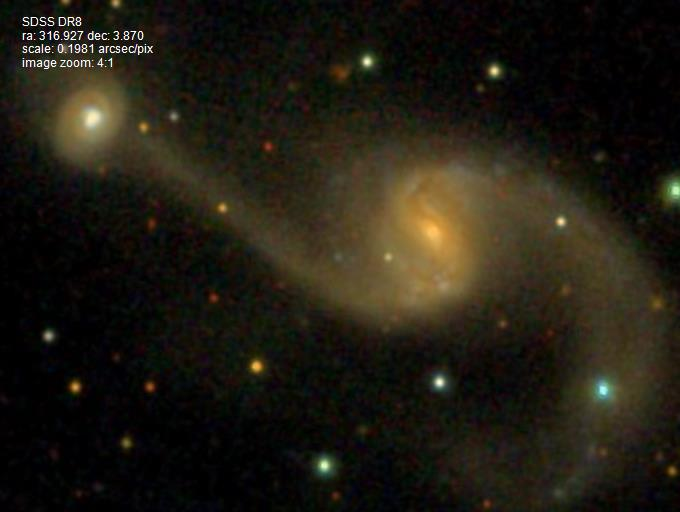
\includegraphics[width=4in]{ugc11680.jpg}
   \caption[ Imagen de UGC11680]
    {Imagen en el óptico de UGC11680 (SDSS8).}
 \label{ugc11680}
 \end{figure}


 \noindent UGC11680 es una espiral SBb con AGN tipo 2, con un color rojo en el óptico, lo que la ubica en la secuencia roja del diagrama color magnitud. Los valores que utilizaremos se encuentran recopilados en la tabla \ref{tab_valores}. Si se requieren otros datos, se darán dentro del texto mismo. Haciendo una búsqueda rápida en la literatura se menciona en 17 artículos hasta la fecha.
 Es incluida por primera vez en \citet{hewitt1991} el cual es un catalogo de objetos cuasi-estelares.
 En los años siguientes, es incluida en diferentes estudios de galaxias \textsl{Seyfert} así
 como catálogos de ellas, por ejemplo \citep{thean2000}; \citep{klimanov2001}; \citep{tran2003}. Es interesante notar el artículo  \citet{moustakas2006}  ya la incluye en el grupo de galaxias peculiares. Prosiguen más estudios sobre poblaciones de galaxias \textsl{Seyfert} hasta que se menciona en la presentación del survey \textbf{CALIFA} \citep{sanchez2012}. Dentro de los artículos de la colaboración de \textbf{CALIFA} se menciona en tres: en estudios de galaxias LINERs \footnote{tipo de galaxia que tiene una emisión nuclear de baja ionización. Esta en debate actual si se considera esta ionización un producto del AGN o simplemente de la emisión de estrellas post-AGB} \citep{singh2013}, en estudios de cinemática de gas en galaxias en proceso de fusión \citep{barrera2015} y su clasificación como barrada para estudiar esta propiedad \citep{blazquez2007}, aunque en el catálogo de NED  UGC11680 está clasificada como Scd, mantendremos la morfología barrada. Una imagen de UGC11680 obtenida de SDSS 8 se muestra en la Figura \ref{ugc11680}.

 \begin{table}[!ht]
 \centering
 \begin{tabular}{||c | c||}
 \hline
 \hline
 Valores Principales & UGC11680NED01 \\
 \hline
 \hline
 Centroide & 36.840,31.753 \\
 Redshift & 0.025887\\
 $R_e$ (kpc) & 8.189 \\
 Log Masa St sin corregir  & 11.337\\
 $H_{\alpha}/H_{\beta}$ & 4.052 \\
 Promedio $A_v$ & 1.092  (mag) \\
 $A_v$ ponderado  & 1.674  (mag) \\
 SFR & 4.143 ($M_{\odot}/yr^2$) \\
 log SFR & 0.617 $\log_{10}$ $(M_{\odot}/yr^2)$ \\
 Ionización Central & sAGN  $>$ Kewley y $|EW (H_{\alpha})|>6$\\
 Velocidad Sist Gas & 7771.840 km/s \\
 Velocidad sistemica SSP & 7749.618 km/s \\
 \hline
 \hline
 \end{tabular}
 \caption[Datos de UGC11680] {Valores Principales UGC11680 (obtenidos de aplicar \textbf{PIPE3D} al cubo de datos de UGC11680)}
 \label{tab_valores}                              %etiqueta para referencia
 \end{table}




%%%%%%%%%%%%%%%%%%%%%%%%%%%%%%%%%%%%%%%%%%%%%%%%%%%%%%%%%%%%%%%%%%%%%%%%%
%                           Objetivo                                    %
%%%%%%%%%%%%%%%%%%%%%%%%%%%%%%%%%%%%%%%%%%%%%%%%%%%%%%%%%%%%%%%%%%%%%%%%%

\section{Objetivos}
En este trabajo nos concentraremos en un solo aspecto para estudiar a la galaxia UGC11680: sus poblaciones estelares  y por lo tanto la información que requerimos para empezar a comprender por que tiene este color rojo.

\bigskip

\noindent Aunque es solo una galaxia, los resultados de su estudio  nos darán pistas para continuar resolviendo y tratando de entender la evolución galáctica y ofrecer un método sólido para su estudio. Por ejemplo, con imágenes multi-banda con buena resolución espacial, es posible resolver la historia de formación estelar en espacio y tiempo, lo que ya ha sido hecho con anterioridad (por ejemplo, \citet{brinchmann2000}; \citet{kong2000}; \citet{perezg2008}) y el llamado método de registro fósil ha sido
ampliamente utilizado para recuperar las historias de formación estelares
utilizando  datos espectrales y fotométricos (\citet{kaufmann2006}; \citet{cid2005}; \citet{gallazzi2005}).
Por otro lado, estos estudios están limitados por el tamaño de la apertura (para el caso de los datos de espectroscopía).
La resolución espectral (en el caso de imágenes multi-banda) pueden generar un sesgo importante en la interpretación de los datos y por consiguiente las conclusiones sobre los procesos evolutivos.

\bigskip

\noindent Es interesante notar que una apertura con tamaño fijo no puede resolver localmente las propiedades de las galaxias debido a que el espectro de la galaxia observada integra toda o una fracción sustancial de la luz dentro de una apertura. Para el caso de los estudios fotométricos, se requiere un número de bandas fotométricas lo suficientemente grandes como para
producir el espectro de galaxias. Sin embargo, con la llegada de la espectroscopía 3D o espectroscopia de campo integral (IFS),  es
posible acceder a los datos espectrales resueltos para diferentes
regiones de galaxias y obtener así espectros locales (por ejemplo, \cite{cappellari2012}; \cite{croom2012}; \cite{sanchez2012}; \cite{cid2013_1}; \cite{bundy2015} ).

\bigskip


\noindent Con datos IFUs y  la descomposición con poblaciones estelares simples (SSP), es factible no sólo
obtener información de como UGC11680 ensambló su  masa estelar, sino también es posible entender la forma en que esta se ensambló a nivel local. Trabajos observacionales recientes indican que una fracción importante
de las galaxias estudiadas tienden a formar la mayor parte de sus masas estelares en su parte interna más rápido que en su exterior,
lo que sugiere que estas galaxias ensamblan sus masas
desde dentro hacia afuera ( \citet{blazquez2007}; \cite{perez2013}) ({\color{red} Ibarra-Medel, et.al. Submitted }).

\bigskip

\noindent Por ejemplo, usando datos de \textbf{CALIFA} \cite{perez2013} mostraron que la velocidad de este proceso
depende de la masa total de la galaxia estelar. Además, hay indicios de
una fase de transición en la que se cambia el crecimiento de masa de las galaxias de dentro hacia afuera
a un gradiente de afuera hacia adentro y que depende de la masa de las galaxias (\cite{perez2013}). Así, es fundamental la comprensión de cómo algunas galaxias apagan su formación de estrellas, lo que regula su crecimiento. Este apagado
se denomina comúnmente en la literatura  como``quenching'', y
podría ser utilizado para explicar la formación y consecuente declinación en formación estelar en UGC11680 durante su evolución.

\bigskip

\noindent Aunque solo se trata de una galaxia, el estudio y manejo comparativo de las historias de formación estelar
son novedosas y no encontradas hasta la fecha en la literatura. Por lo tanto,
en análisis futuros se podría utilizar este método para una muestra mas significativa de galaxias.
Al poder utilizar métodos que nos permiten observar las épocas de formación galáctica, daremos un paso adelante para contribuir
en el análisis y posiblemente utilizarlo en diferentes variables de interés.

\bigskip


\subsection{Estructura de la tesis}

Este trabajo está dividido en 3 Capítulos y un apéndice, y se explican como sigue:

\begin{itemize}

\item El primer capítulo incluye la introducción, donde incluimos los antecedentes generales del estudio de objetos extra-galactico, la definición de AGN y sus propiedades esenciales; una breve discusión sobre la bimodalidad y el estado del arte como diagrama evolutivo. Presentamos además a la galaxia UGC11680 y sus características principales.


\item En el siguiente capitulo se explicará brevemente el muestreo de \textbf{CALIFA}, que son los IFUs y el proceso de análisis de los cubos y los datos que se obtengan de ellos. Después haremos un chequeo general del enrojecimiento  por polvo y analizaremos la tasa de formación estelar de UGC11680 con respecto a las galaxias de la muestra. Una vez descartado el enrojecimiento por polvo, explicaremos el proceso para obtener las poblaciones estelares y que servirán para obtener el producto final, la historia de formación estelar con su mapa $SFH(t,R)$; Esto es importante, ya que todo nuestro análisis posterior depende de este parámetro.

\item El capítulo final incluirá el análisis sobre la historia de formación estelar espacialmente resuelta para la galaxia UGC11680 y para diferentes tipos de galaxias, promediadas en diferentes categorías. Se compararán estas historias en base al parámetro  $\chi^2$ y esto nos indicará a que promedios se parece ó ajusta más UGC11680 con respecto a su historia de formación estelar.

\item Finalmente incluimos un breve apéndice en donde se incluye por que sabemos que UGC11680 es una galaxia con AGN.

\end{itemize}

\noindent La galaxia de estudio UGC11680 se dividió en 3 zonas de estudio determinadas por su radio efectivo. A lo largo de esta tesis, llamamos ``partes centrales'' a la zona comprendida por $0< R/R_e < 0.5$, ``partes medias'' a la zona $ 0.5< R/R_e < 1.25 $ y las zonas externas o las ``afueras'' a $1.25<R/R_e < 2.0$.

\bigskip

\noindent Finalmente, en este trabajo los parámetros cosmológicos utilizados fueron $\Omega_m = 0.317$ , $\Omega_{\Lambda}=0.683$ y $H_0 = 67.15$ km/s/Mpc \citep{plank2014}

